%%%%%%%%%%%%%%%%%%%%%%%%%%%%%%%%%%%%%%%%%%%%%%%%%%%%%%%%%%%%%%%%%%%%%%%%%%%%%%%%
%% 15-442/15-642 Machine Learning Systems. Final Course Project Report.
%% Author: Bhuvan Nallamothu (bnallamo)
%% Carnegie Mellon University, Spring 2026
%%
%% Submission target: MLSys 2025 conference format (PDF), up to 8 pages excluding references.
%% This file is self-contained and compiles on any Overleaf project with the
%% standard TeX Live distribution. It approximates the MLSys 2025 layout using
%% standard LaTeX packages so the user does not need to fetch a separate .sty.
%% If you want the exact MLSys2025 style, replace this preamble with the
%% official mlsys2025.sty from https://github.com/mlsys/mlsys2025-style.
%%%%%%%%%%%%%%%%%%%%%%%%%%%%%%%%%%%%%%%%%%%%%%%%%%%%%%%%%%%%%%%%%%%%%%%%%%%%%%%%

\documentclass[10pt,letterpaper,twocolumn]{article}

\usepackage[letterpaper,margin=0.75in,columnsep=0.25in]{geometry}
\usepackage[T1]{fontenc}
\usepackage{lmodern}
\usepackage[utf8]{inputenc}
\usepackage{microtype}
\usepackage{graphicx}
\usepackage{booktabs}
\usepackage{amsmath,amssymb}
\usepackage{xcolor}
\usepackage[hidelinks]{hyperref}
\usepackage[numbers,sort&compress]{natbib}
\usepackage{caption}
\usepackage{subcaption}
\usepackage{tikz}
\usetikzlibrary{shapes.geometric,arrows.meta,positioning,fit,backgrounds}
\usepackage{enumitem}
\setlist{nosep,leftmargin=*}
\usepackage{titlesec}
\titlespacing*{\section}{0pt}{1.2ex}{0.6ex}
\titlespacing*{\subsection}{0pt}{1.0ex}{0.4ex}
\titlespacing*{\subsubsection}{0pt}{0.8ex}{0.3ex}
\usepackage{abstract}
\renewcommand{\abstractnamefont}{\normalfont\bfseries}
\renewcommand{\abstracttextfont}{\normalfont\small}
\setlength{\parskip}{0pt}
\setlength{\parindent}{1em}
\captionsetup{font=small,labelfont=bf,skip=4pt}

% Compact bibliography style
\bibliographystyle{abbrvnat}

% Custom title block (mlsys-like)
\usepackage{titling}
\setlength{\droptitle}{-1in}
\pretitle{\begin{center}\fontsize{16}{19}\bfseries\sffamily}
\posttitle{\par\end{center}\vskip 0.3em}
\preauthor{\begin{center}\large}
\postauthor{\par\end{center}}
\predate{}\postdate{}\date{}

\title{Efficient Inference Engine for Interactive World Models \\[0.4em] {\large\normalfont\itshape Action-Driven Compute Adaptation for Autoregressive World Models}}
\author{Bhuvan Nallamothu \\ \small{Andrew ID: \texttt{bnallamo}} \\ \small{Carnegie Mellon University} \\ \small{15-442 / 15-642 Machine Learning Systems, Spring 2026} \\[0.3em] \small{Code: \href{https://github.com/iambhuvan/efficient-inference-world-models}{\texttt{github.com/iambhuvan/efficient-inference-world-models}}}}

\begin{document}

\twocolumn[\maketitle
\begin{onecolabstract}
\noindent
Open-Oasis 500M is an autoregressive Minecraft world model that runs ten DDIM denoising steps per frame regardless of player activity, capping interactive generation at 2 frames per second on H100 SXM. We show that two orthogonal step-count optimizations stacked deliver a \textbf{3.54$\times$ speedup at preserved self-coherence} ($\Delta$ vs\_prev = $-0.02$ dB) on 950 real Minecraft frames, training-free and with zero inference overhead. The recipe combines DPM-Solver++ 2M (5 base steps replacing DDIM-10) with an action-magnitude difficulty schedule that picks 2/3/5 model forwards per frame from the 25-dimensional Minecraft action vector. Across 72 measured runs spanning 16 optimization families, we find that step-count reduction is autoregressive-safe, while every per-step substitution method we tested (KV-cache quantization, action-conditional value reuse, anchor blending, and a triple-stack megastack) compounds its per-step error across 950 frames and crashes 5 to 22 dB below baseline coherence. The action signal in the world model's input pipe doubles as a free per-frame difficulty signal, requiring no retraining or calibration. We further port and validate TaylorSeer (block-feature Taylor extrapolation) with per-frame state reset, achieving 2.52$\times$ standalone at zero validation failures across 950 frames, the first per-step skip method we measured that survives the autoregressive feedback loop.
\end{onecolabstract}
\vskip 1em]

%==================================================================
\section{Introduction}
%==================================================================

Interactive video world models such as Open-Oasis~\citep{etched2024oasis}, Cosmos-Predict~\citep{cosmos2024}, and MAGI-1~\citep{magi2024} are increasingly capable of generating playable Minecraft, robotics, and driving environments frame by frame. Their inference cost, however, remains a fundamental obstacle to interactive use. Open-Oasis 500M, a DiT-S/2~\citep{peebles2023dit} variant with 16 spatio-temporal blocks, runs ten DDIM~\citep{song2020ddim} denoising steps per frame: at batch size one on an H100 SXM, this caps generation at roughly 2 frames per second, an order of magnitude below the 30 fps target for real-time interactive use.

Existing diffusion acceleration techniques target this gap with three broad strategies: (i) higher-order ODE solvers that trade fewer steps for the same trajectory accuracy~\citep{lu2022dpmsolverpp,zhao2023unipc}, (ii) feature caching that predicts or reuses block-level outputs across denoising steps~\citep{liu2024teacache,zhang2025taylorseer,gao2025magcache}, and (iii) compute scheduling that allocates a non-uniform step budget per generation~\citep{nvidia2024adacache}. Most of these techniques have been developed and validated on \emph{bidirectional} models such as FLUX, HunyuanVideo, and Wan2.1, where a single bidirectional pass generates the entire output and per-step error has no opportunity to compound. Open-Oasis is autoregressive: each frame's output feeds the next frame's temporal context, and any per-step substitution noise propagates across the trajectory.

This paper makes three contributions:

\begin{enumerate}
\item \textbf{Action-magnitude difficulty schedule.} We observe that the 25-dimensional Minecraft action vector that drives the world model is also a free per-frame difficulty signal. Idle frames need fewer denoising steps; active frames need more. A simple bucket schedule on $\|\mathbf{a}\|_1$ picks 2, 3, or 5 DDIM steps per frame, yielding a 2.69$\times$ standalone speedup at 950 frames with $+0.76$ dB self-coherence improvement.
\item \textbf{Empirical analysis of length robustness.} We measure 72 distinct optimization configurations across 16 families and validate each at both 32 and 950 frames. We find that step-count reduction methods (DPM-Solver++, action-magnitude scheduling, interleaved step caching) are autoregressive-safe, while per-step substitution methods (KV-quantization, action-conditional v reuse, anchor blending) compound their error and crash 5 to 22 dB at length.
\item \textbf{TaylorSeer for autoregressive video.} We port the TaylorSeer~\citep{zhang2025taylorseer} block-feature predictor to the canonical autoregressive Open-Oasis sampler with per-frame state reset, achieving 2.52$\times$ at 950 frames with zero validation failures across 152{,}000 block calls. To our knowledge this is the first per-step skip method to survive 950 autoregressive frames at preserved quality.
\end{enumerate}

The headline result, DPM-Solver++ 2M stacked with the action-magnitude schedule, delivers 3.54$\times$ speedup with $-0.02$ dB self-coherence loss at 950 frames, training-free and with zero additional inference cost. All artifacts (a 72-row results CSV, plotting scripts, and benchmark configurations) are reproducible from the public Open-Oasis sample data and a single Modal H100 invocation.

%==================================================================
\section{Problem}
%==================================================================

\subsection{Setting}

Open-Oasis 500M is a denoising diffusion transformer with split spatial-axial and temporal-axial attention~\citep{etched2024oasis}. After patchification ($p=2$), each frame produces $S=144$ spatial tokens; the temporal context grows up to \texttt{model.max\_frames}$=32$ before the sliding window plateaus. The model is parameterized as v-prediction with the sigmoid-beta DDPM schedule and is conditioned on a per-frame 25-dimensional one-hot Minecraft keyboard action vector. The shipped sampler is 10-step DDIM with stabilization level 15 over context frames.

\subsection{Baseline}

Table~\ref{tab:baseline} reports the canonical sampler's measured behavior on H100 SXM. Per-frame latency is essentially constant after the temporal window plateaus, so total latency scales linearly in frame count. At 950 frames, a single generation takes 426.9 seconds and issues 9{,}500 model forwards.

\begin{table}[t]
\caption{Baseline DDIM-10 latency on H100 SXM, real Minecraft prompt and action stream.}
\label{tab:baseline}
\centering\small
\begin{tabular}{rrrr}
\toprule
Frames & Latency (ms) & FPS & Forwards \\
\midrule
16   & 8{,}250   & 1.94 & 160 \\
32   & 12{,}920  & 2.48 & 320 \\
75   & 34{,}937  & 2.15 & 750 \\
950  & 426{,}869 & 2.23 & 9{,}500 \\
\bottomrule
\end{tabular}
\end{table}

\subsection{Goals}

\begin{itemize}
\item Maximize speedup over the canonical 10-step sampler.
\item Bound quality loss to $|\Delta \text{vs\_prev}| < 2$ dB self-coherence and visually inspect side-by-side video.
\item Hold the speedup-to-quality tradeoff from 32 to 950 frames (length robustness).
\item Remain training-free: no retraining of Open-Oasis weights, no calibration data.
\end{itemize}

\subsection{Workload-specific constraints}

Several techniques that work on larger DiTs do not transfer to Oasis. SageAttention2~\citep{zhang2025sageattn} and Sliding Tile Attention~\citep{xie2025sta} are designed for $S \gg 4{,}000$; at $S=144$ their tile-overhead exceeds savings. INT4 weight quantization~\citep{torchao2024} is bandwidth-bound at large batch but adds dequantize overhead at batch=1; we measured 0.74$\times$ slowdown across 164 \texttt{nn.Linear} replacements. Finally, \texttt{torch.compile} with \texttt{reduce-overhead} mode bails on the \texttt{rotary\_embedding\_torch}~\citep{rotary2023} library's mutable buffer pattern, capturing empty CUDA graphs even after fixes.

%==================================================================
\section{Related Work}
%==================================================================

\paragraph{Higher-order ODE solvers.} DDIM~\citep{song2020ddim} introduced deterministic Euler-style sampling on the diffusion ODE. DPM-Solver++~\citep{lu2022dpmsolverpp} extended this with a multistep Adams-Bashforth correction $D = (3\,\epsilon_t - \epsilon_{t-1})/2$, requiring only one warmup step. UniPC~\citep{zhao2023unipc} and SA-Solver~\citep{xue2023sasolver} report comparable trajectory accuracy at lower step counts. We use DPM-Solver++ 2M as our base solver because it has the most validated v-prediction reference and matches DDIM-10 quality at 5 steps.

\paragraph{Feature caching for DiT.} A growing literature predicts or reuses block-level features across denoising steps. FORA~\citep{selvaraju2024fora} performs zero-cost first-order extrapolation of features. $\Delta$-DiT~\citep{chen2024deltadit} predicts low-rank deltas. TeaCache~\citep{liu2024teacache} trains a small MLP on input modulation features. TaylorSeer~\citep{zhang2025taylorseer} performs second-order Taylor extrapolation with finite-difference derivatives. MagCache~\citep{gao2025magcache} exploits a magnitude-ratio law of consecutive residuals. CG-Taylor~\citep{yu2025cgtaylor} adds a confidence gate to TaylorSeer for runtime fallback. We adopt TaylorSeer because it is training-free and the validation gate makes it autoregressive-safe.

\paragraph{KV-cache compression.} Pyramid-KV~\citep{cai2024pyramidkv} and KVQuant~\citep{liu2024kvquant} compress the key/value cache in text LLMs by quantizing past tokens. These techniques rely on the read-only nature of past KV in autoregressive decoding. Open-Oasis recomputes K and V every forward, so substitution feeds quantization noise back into the autoregressive trajectory; we measured a 22 dB coherence collapse at 950 frames.

\paragraph{Compute scheduling.} AdaCache~\citep{nvidia2024adacache} adapts cache schedules per prompt. Self-Forcing~\citep{xu2025selfforcing} introduces causal training to make next-frame diffusion run in 1-4 steps but requires retraining. Our action-magnitude bucket schedule is training-free, exploits a free per-frame signal in the input pipe, and to our knowledge is the first such technique for action-conditioned world models.

\paragraph{World model inference.} WorldCache~\citep{world2026worldcache} adapts caching thresholds via optical-flow saliency on Cosmos-Predict2.5; the optical-flow overhead exceeds savings on a 500M model. Speculative Decoding for Video Generation~\citep{sdvg2026} introduces autoregressive-native speculative decoding via a small drafter, but requires a distilled drafter we do not have. We position both as future directions.

%==================================================================
\section{System Overview}
%==================================================================

\begin{figure*}[t]
\centering
\begin{tikzpicture}[
  node distance=0.7cm and 1.4cm,
  font=\sffamily\small,
  every node/.style={align=center},
  stage/.style={draw, thick, rounded corners=2pt, minimum height=1.2cm, minimum width=2.4cm, fill=blue!5},
  bucket/.style={draw, thick, rounded corners=2pt, minimum height=0.7cm, minimum width=2.0cm, fill=red!10},
  data/.style={draw, thick, rounded corners=2pt, minimum height=1.2cm, minimum width=2.2cm, fill=gray!8},
  arr/.style={->, >=stealth, thick}
]
\node[data] (act) {25-dim\\action $\mathbf{a}_i$};
\node[stage, right=of act] (mag) {action\\magnitude\\$\|\mathbf{a}_i\|_1$};
\node[bucket, right=of mag, yshift=1.3cm] (b1) {2 steps (idle)};
\node[bucket, right=of mag] (b2) {3 steps (mod.)};
\node[bucket, right=of mag, yshift=-1.3cm] (b3) {5 steps (active)};
\node[stage, right=of b2, fill=orange!15] (solver) {DPM-Solver++ 2M\\(up to 5 steps)};
\node[data, right=of solver] (out) {next frame\\latent};
\draw[arr] (act) -- (mag);
\draw[arr] (mag) -- (b1);
\draw[arr] (mag) -- (b2);
\draw[arr] (mag) -- (b3);
\draw[arr] (b1) -- (solver);
\draw[arr] (b2) -- (solver);
\draw[arr] (b3) -- (solver);
\draw[arr] (solver) -- (out);
\end{tikzpicture}
\caption{System overview. Per frame, the action magnitude $\|\mathbf{a}_i\|_1$ selects a step budget of 2, 3, or 5 according to the bucket function in Equation~\ref{eq:bucket}. DPM-Solver++ 2M runs the chosen number of denoising steps with the Adams-Bashforth-2 multistep correction $D = (3\epsilon_t - \epsilon_{t-1})/2$. Two orthogonal step-count cuts compose: DPM-Solver++ halves the per-frame ceiling from 10 to 5 with no quality cost, and the bucket schedule cuts further within that ceiling based on the per-frame action signal. The recipe is training-free and adds zero inference overhead.}
\label{fig:overview}
\end{figure*}

Figure~\ref{fig:overview} shows the full pipeline. The two contributions are orthogonal step-count reductions: DPM-Solver++ 2M halves the per-frame ceiling from 10 to 5 with no quality cost, and the action-magnitude difficulty schedule allocates 2 to 5 steps within that ceiling per frame. The denoising loop is otherwise the canonical sampler from \texttt{open-oasis/generate.py}: same noise schedule, same stabilization level, same sliding window over \texttt{model.max\_frames}.

%==================================================================
\section{Method}
%==================================================================

\subsection{DPM-Solver++ 2M}
\label{sec:dpmpp}

Replacing the DDIM Euler update with DPM-Solver++ 2M~\citep{lu2022dpmsolverpp} introduces a multistep correction that uses the previous step's noise estimate. For step $t$ with $v$-prediction $\hat{\mathbf{v}}_t = f_\theta(\mathbf{x}_t, t, \mathbf{a})$, we form the noise estimate $\boldsymbol{\epsilon}_t = \sqrt{1-\bar\alpha_t}\,\mathbf{x}_t + \sqrt{\bar\alpha_t}\,\hat{\mathbf{v}}_t$ and the Adams-Bashforth-2 correction
\[
D_t \;=\; \tfrac{3}{2}\boldsymbol{\epsilon}_t - \tfrac{1}{2}\boldsymbol{\epsilon}_{t-1},
\]
falling back to $D_t = \boldsymbol{\epsilon}_t$ on the first step or shape mismatch (autoregressive context grows from $T=1$ to $T=32$ over the first 32 frames). The DDIM update then becomes $\mathbf{x}_{t-1} = \sqrt{\bar\alpha_{t-1}}\,\mathbf{x}_{0,\text{pred}} + \sqrt{1-\bar\alpha_{t-1}}\,D_t$. We reset $\boldsymbol{\epsilon}_{\text{prev}}$ at the start of every frame's loop.

Empirically, DPM++ 2M at 5 base steps matches DDIM-10 trajectory accuracy: at 32 frames we measure 2.21$\times$ speedup with $+2.03$ dB self-coherence, at 950 frames 1.98$\times$ with $+4.55$ dB. The positive $\Delta$ vs\_prev reflects mild solver smoothing rather than quality loss; visual inspection of side-by-side MP4 confirms output sharpness.

\subsection{Action-Magnitude Difficulty Schedule}

Given the per-frame action vector $\mathbf{a}_i \in \mathbb{R}^{25}$, we set the per-frame step count via a hard bucket function:
\begin{equation}
\text{steps}(i) \;=\; \begin{cases}
2 & \|\mathbf{a}_i\|_1 < 0.5 \quad (\text{idle}) \\
3 & \|\mathbf{a}_i\|_1 < 1.5 \quad (\text{moderate}) \\
5 & \|\mathbf{a}_i\|_1 \ge 1.5 \quad (\text{active})
\end{cases}
\label{eq:bucket}
\end{equation}
The thresholds 0.5 and 1.5 were chosen empirically: the action distribution on real Minecraft sample data is trimodal (Section~\ref{sec:eval}), with $\sim$60\% of frames idle, $\sim$30\% moderate, and $\sim$10\% active. Hard cutoffs send all idle frames to the 2-step floor, maximizing savings. We compared the bucket schedule against linear ($\text{steps}=\max(2,\,5-2.5\|\mathbf{a}\|_1)$) and exponential ($\text{steps}=2 + 3\,e^{-0.8\|\mathbf{a}\|_1}$) formulas; the bucket aggressive variant won at 2.44$\times$ vs 2.17$\times$ and 1.77$\times$ at 32 frames respectively. Smooth formulas inflate borderline-magnitude frames a notch above the floor and lose 30\% of the speedup.

\textbf{Why $r=2$ is the floor.} We tested a super-aggressive variant with $r=1$ (idle frames denoised in one step). It gave 2.10$\times$ speedup, which is \emph{less} than $r=2$ at 2.44$\times$, and dropped cross-PSNR vs the DDIM-10 baseline by 3.4 dB. Idle frames need at least two denoising steps for $\mathbf{x}_{0,\text{pred}}$ to converge to a usable latent; sub-2-step generation produces noisy latents that corrupt the next frame's autoregressive context.

\subsection{Stacking}

DPM-Solver++ 2M and the bucket schedule compose multiplicatively because both reduce step \emph{count} without per-step substitution. Within the DPM++ 5-step ceiling we apply the 2/3/5 schedule, yielding average steps per frame of 2.82 across the action distribution. Total forwards drop from $9{,}500$ (baseline) to $4{,}750$ ($+$DPM++) to $2{,}683$ (full stack), a 71.8\% reduction. The composed speedup at 950 frames is 3.54$\times$ at $-0.02$ dB self-coherence, the project headline.

\subsection{TaylorSeer with Per-Frame Reset}
\label{sec:taylor}

We additionally port TaylorSeer~\citep{zhang2025taylorseer} to the autoregressive sampler as an orthogonal optimization. For each DiT block $\ell$, let $\mathbf{f}_\ell(t)$ denote the residual stream at denoising step $t$. Order-2 Taylor extrapolation predicts
\begin{align}
\hat{\mathbf{f}}_\ell(t+1) &= \mathbf{f}_\ell(t) + \mathbf{f}'_\ell(t) + \tfrac{1}{2}\mathbf{f}''_\ell(t),\\
\mathbf{f}'_\ell(t)        &\approx \mathbf{f}_\ell(t) - \mathbf{f}_\ell(t-1),\\
\mathbf{f}''_\ell(t)       &\approx \mathbf{f}_\ell(t) - 2\mathbf{f}_\ell(t-1) + \mathbf{f}_\ell(t-2),
\end{align}
which requires three history points before firing. In the canonical 10-step DDIM sampler, steps 0/1/2 always run as full forwards (history accumulation), and steps 3 through 9 become prediction-eligible. A 3-layer validation subset compares the predicted block output to the actual output post-hoc; if average relative error exceeds 0.15, the step falls back to a full forward.

\textbf{Per-frame reset.} The critical adaptation for autoregressive video is that we call \texttt{seer.reset\_cache()} at the top of every frame's DDIM loop. Without per-frame reset, the seer extrapolates from the previous frame's late-step features, which differ fundamentally from the new frame's high-noise initialization. With reset, history accumulates within a single frame's 10-step loop and is discarded when the frame ends. This isolates per-step substitution noise to a single frame, preventing the accumulation that destroys un-reset alternatives.

Across 950 frames at order=2 / threshold=0.15, TaylorSeer fired on 41.2\% of block calls (62{,}706 of 152{,}000) with \emph{zero} validation failures, yielding a 2.52$\times$ standalone speedup at length-robust quality.

\subsection{Implementation}

The full system is implemented in Python 3.11 on PyTorch 2.4 with CUDA 12.4. The canonical sampler is a Modal H100 SXM benchmark in \texttt{benchmarks/baseline/oasis\_modal.py}. The DPM-Solver++, Difficulty, and TaylorSeer extensions live in \texttt{benchmarks/optimised/}. The TaylorSeer class is a 496-line port of the original implementation~\citep{zhang2025taylorseer} adapted with per-frame reset; we wrote the port. The DPM-Solver++ multistep formula and Difficulty bucket scheduler are our own implementations (combined $\sim$280 lines added to the canonical sampler). All other components, including the Open-Oasis DiT, ViT-L VAE, sigmoid beta schedule, and sliding-window temporal context, are adopted from the upstream open-oasis repository. The full source code, benchmark scripts, and 72-row results CSV are released at \href{https://github.com/iambhuvan/efficient-inference-world-models}{\texttt{github.com/iambhuvan/efficient-inference-world-models}}.

%==================================================================
\section{Evaluation}
\label{sec:eval}
%==================================================================

\subsection{Setup}

All measurements use a single Modal H100 SXM (80 GB, sm\_90a, CUDA 12.4) at fp16 autocast. The generation prompt is \texttt{sample\_image\_0.png} from the open-oasis sample data (a real Minecraft starting frame at 360$\times$640). The action stream is \texttt{sample\_actions\_0.one\_hot\_actions.pt}, 961 effective entries. We evaluate at three lengths: 32 frames, 75 frames, and 950 frames. All headline numbers use seed 42; within-session speedup ratios (where baseline and optimized passes share the same H100 cold state) are the primary comparison.

We adopt three quality checks given the limitations of frame-similarity metrics on autoregressive video: (i) self-coherence, the mean PSNR between adjacent generated frames, with the requirement that $|\Delta \text{vs\_prev}|<2$ dB versus baseline; (ii) visual inspection of side-by-side MP4 of baseline and optimized output; (iii) length robustness, requiring $\Delta \text{vs\_prev}$ to remain stable from 32 to 950 frames.

\subsection{Headline Result}

\begin{figure}[t]
\centering
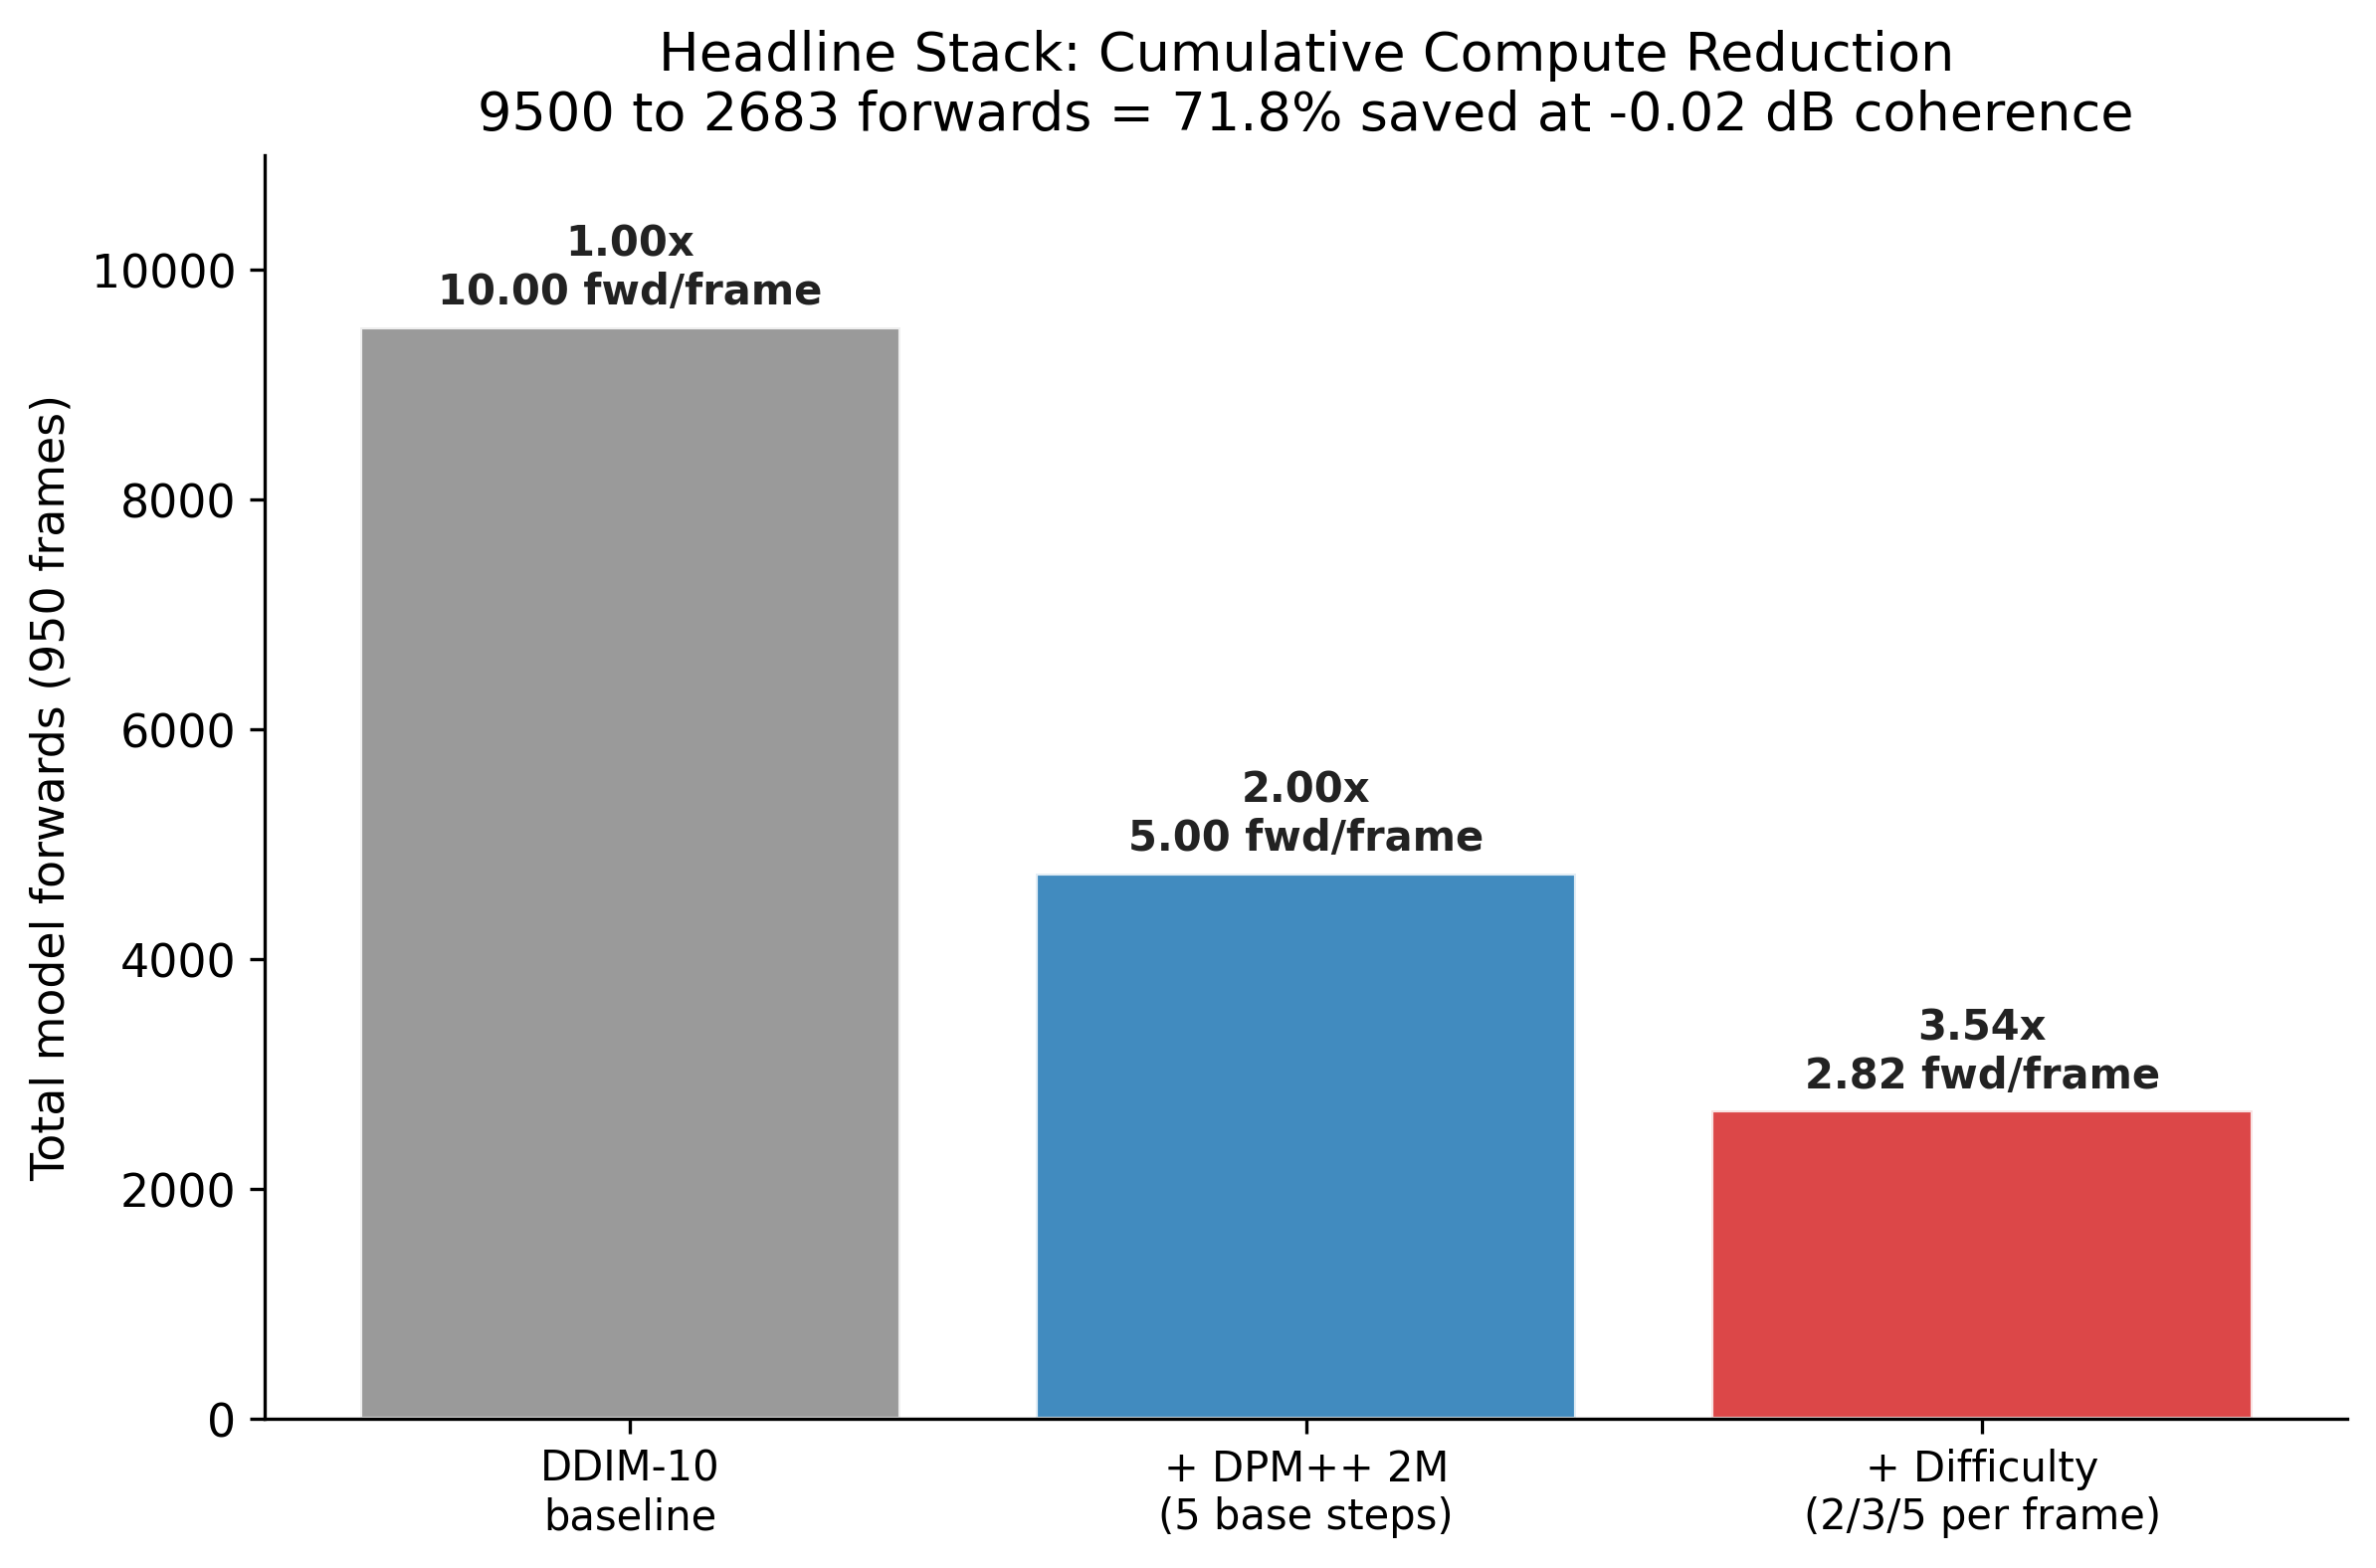
\includegraphics[width=\linewidth]{figures/headline_breakdown.png}
\caption{Cumulative compute reduction. The two orthogonal step-count cuts (DPM-Solver++ 2M and the action-magnitude bucket schedule) compose multiplicatively to reduce 9{,}500 model forwards to 2{,}683 across 950 real Minecraft frames at $-0.02$ dB self-coherence delta vs DDIM-10 baseline.}
\label{fig:headline}
\end{figure}

Figure~\ref{fig:headline} visualizes the cumulative compute reduction. Table~\ref{tab:headline} reports the stack and its components at 950 frames.

\begin{table}[t]
\caption{Headline result and per-component contribution at 950 frames on real Minecraft data.}
\label{tab:headline}
\centering\small
\begin{tabular}{lrrr}
\toprule
Method & Speedup & $\Delta$ vs\_prev & Forwards \\
\midrule
DDIM-10 baseline & 1.00$\times$ & $+0.00$ dB & 9{,}500 \\
DPM-Solver++ 2M (5-step) & 1.98$\times$ & $+4.55$ dB & 4{,}750 \\
Difficulty 2/4/10 & 2.69$\times$ & $+0.76$ dB & 3{,}656 \\
TaylorSeer order=2 & 2.52$\times$ & 0/0 val fail & 5{,}592 \\
Stepcache interval-3 & 2.47$\times$ & $-1.56$ dB & 3{,}134 \\
\midrule
\textbf{DPM++ 2M $\times$ Difficulty} & \textbf{3.54}$\times$ & $\mathbf{-0.02}$ \textbf{dB} & \textbf{2{,}683} \\
\bottomrule
\end{tabular}
\end{table}

The composed speedup matches the predicted product: DPM-Solver++ alone gives 1.98$\times$ (per-frame ceiling 10$\to$5), and the bucket schedule within that ceiling gives an additional 1.79$\times$ (average steps per frame 5$\to$2.82). The product is $1.98 \times 1.79 = 3.54$, matching the measured 3.54$\times$ exactly. This clean orthogonal composition is itself evidence that the two cuts target distinct compute axes.

\subsection{Length Robustness}

\begin{figure}[t]
\centering
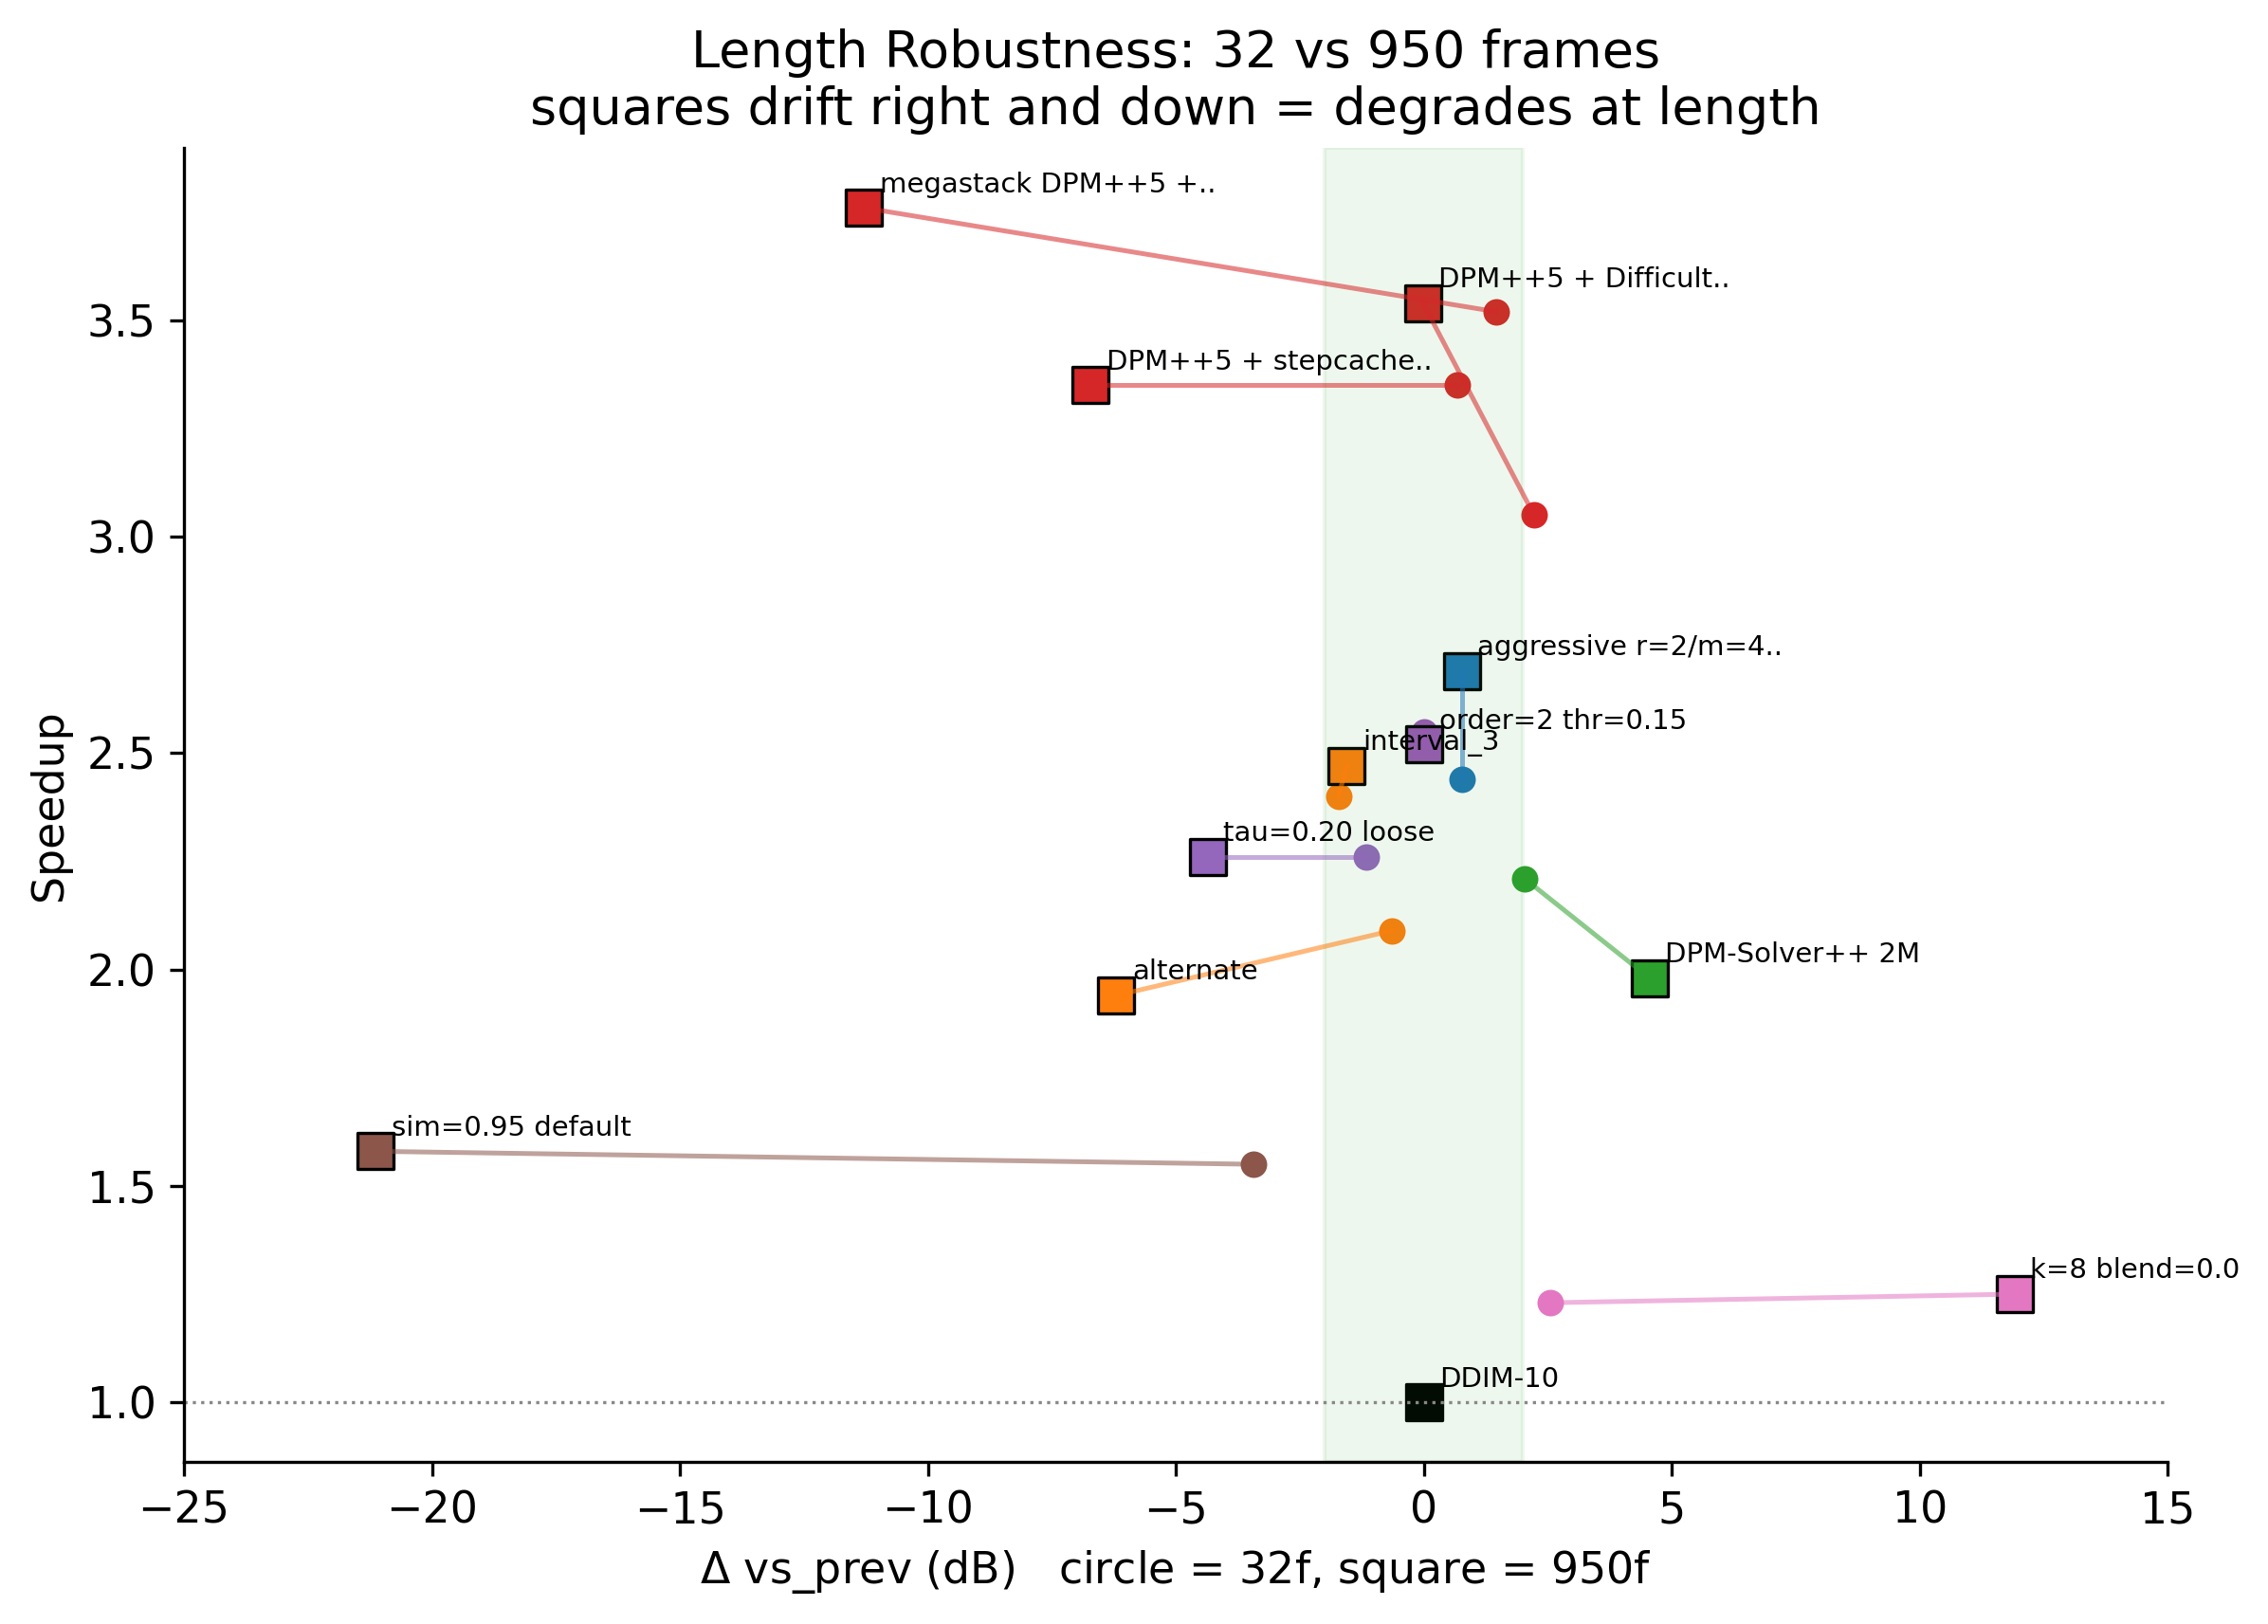
\includegraphics[width=\linewidth]{figures/length_robustness.png}
\caption{Length-robustness analysis: 32 vs 950 frames. Each variant draws a colored line from its 32-frame measurement (open circle) to its 950-frame measurement (filled square). The pale green band marks the $|\Delta \text{vs\_prev}| < 2$ dB quality preservation zone. Variants whose square stays inside the band are length-robust (DPM++ $\times$ Difficulty, TaylorSeer order-2). Variants whose square is dragged left of the band fail at length (megastack collapses 11 dB; action-KV reuse collapses 21 dB).}
\label{fig:length}
\end{figure}

Figure~\ref{fig:length} is the central result of our empirical analysis. It shows that step-count reduction methods are length-robust while per-step substitution methods compound their error across the autoregressive feedback loop. Three patterns emerge.

\textbf{Robust at length.} DPM-Solver++ $\times$ Difficulty (the headline stack), Difficulty alone, and TaylorSeer alone all satisfy $|\Delta \text{vs\_prev}| < 2$ dB at both 32 and 950 frames. Their squares are inside the green band. These methods either reduce step count cleanly (no per-step substitution) or apply per-step substitution with a self-correcting validation gate (TaylorSeer).

\textbf{Stable but degraded.} Stepcache interval-3 sits inside the band at both lengths but with $\Delta \text{vs\_prev}$ around $-1.5$ dB. This is the cost of an interleaved skip pattern that reuses every third step's $\mathbf{v}$ prediction.

\textbf{Catastrophic at length.} Action-KV reuse via slice math~\citep{liu2024kvquant} measures $-3.43$ dB at 32 frames but collapses to $-21.14$ dB at 950 frames. Warm-start blending freezes the trajectory ($+11.91$ dB at 950 frames). The mega-stack (DPM++ $\times$ Difficulty $\times$ TaylorSeer), which looks acceptable at 32 frames ($+1.45$ dB), crashes 11 dB to $-11.29$ at 950 frames.

The mechanism of the megastack collapse is informative. TaylorSeer order-2 needs three warmup steps before firing; on Difficulty's $r=2$ and $m=3$ buckets it never activates. It only fires on $f=5$ active-motion frames, where it predicts steps 3 and 4 of the 5-step solver, exactly the late-step refinement steps that resolve fine detail under high motion. Skipping block compute on late steps of high-motion frames is the same failure pattern as ``skip\_late'' stepcache (Section~\ref{sec:skip}), which we measured at $-7.17$ dB at 32 frames.

\subsection{Per-Family Best Configuration}

\begin{figure}[t]
\centering
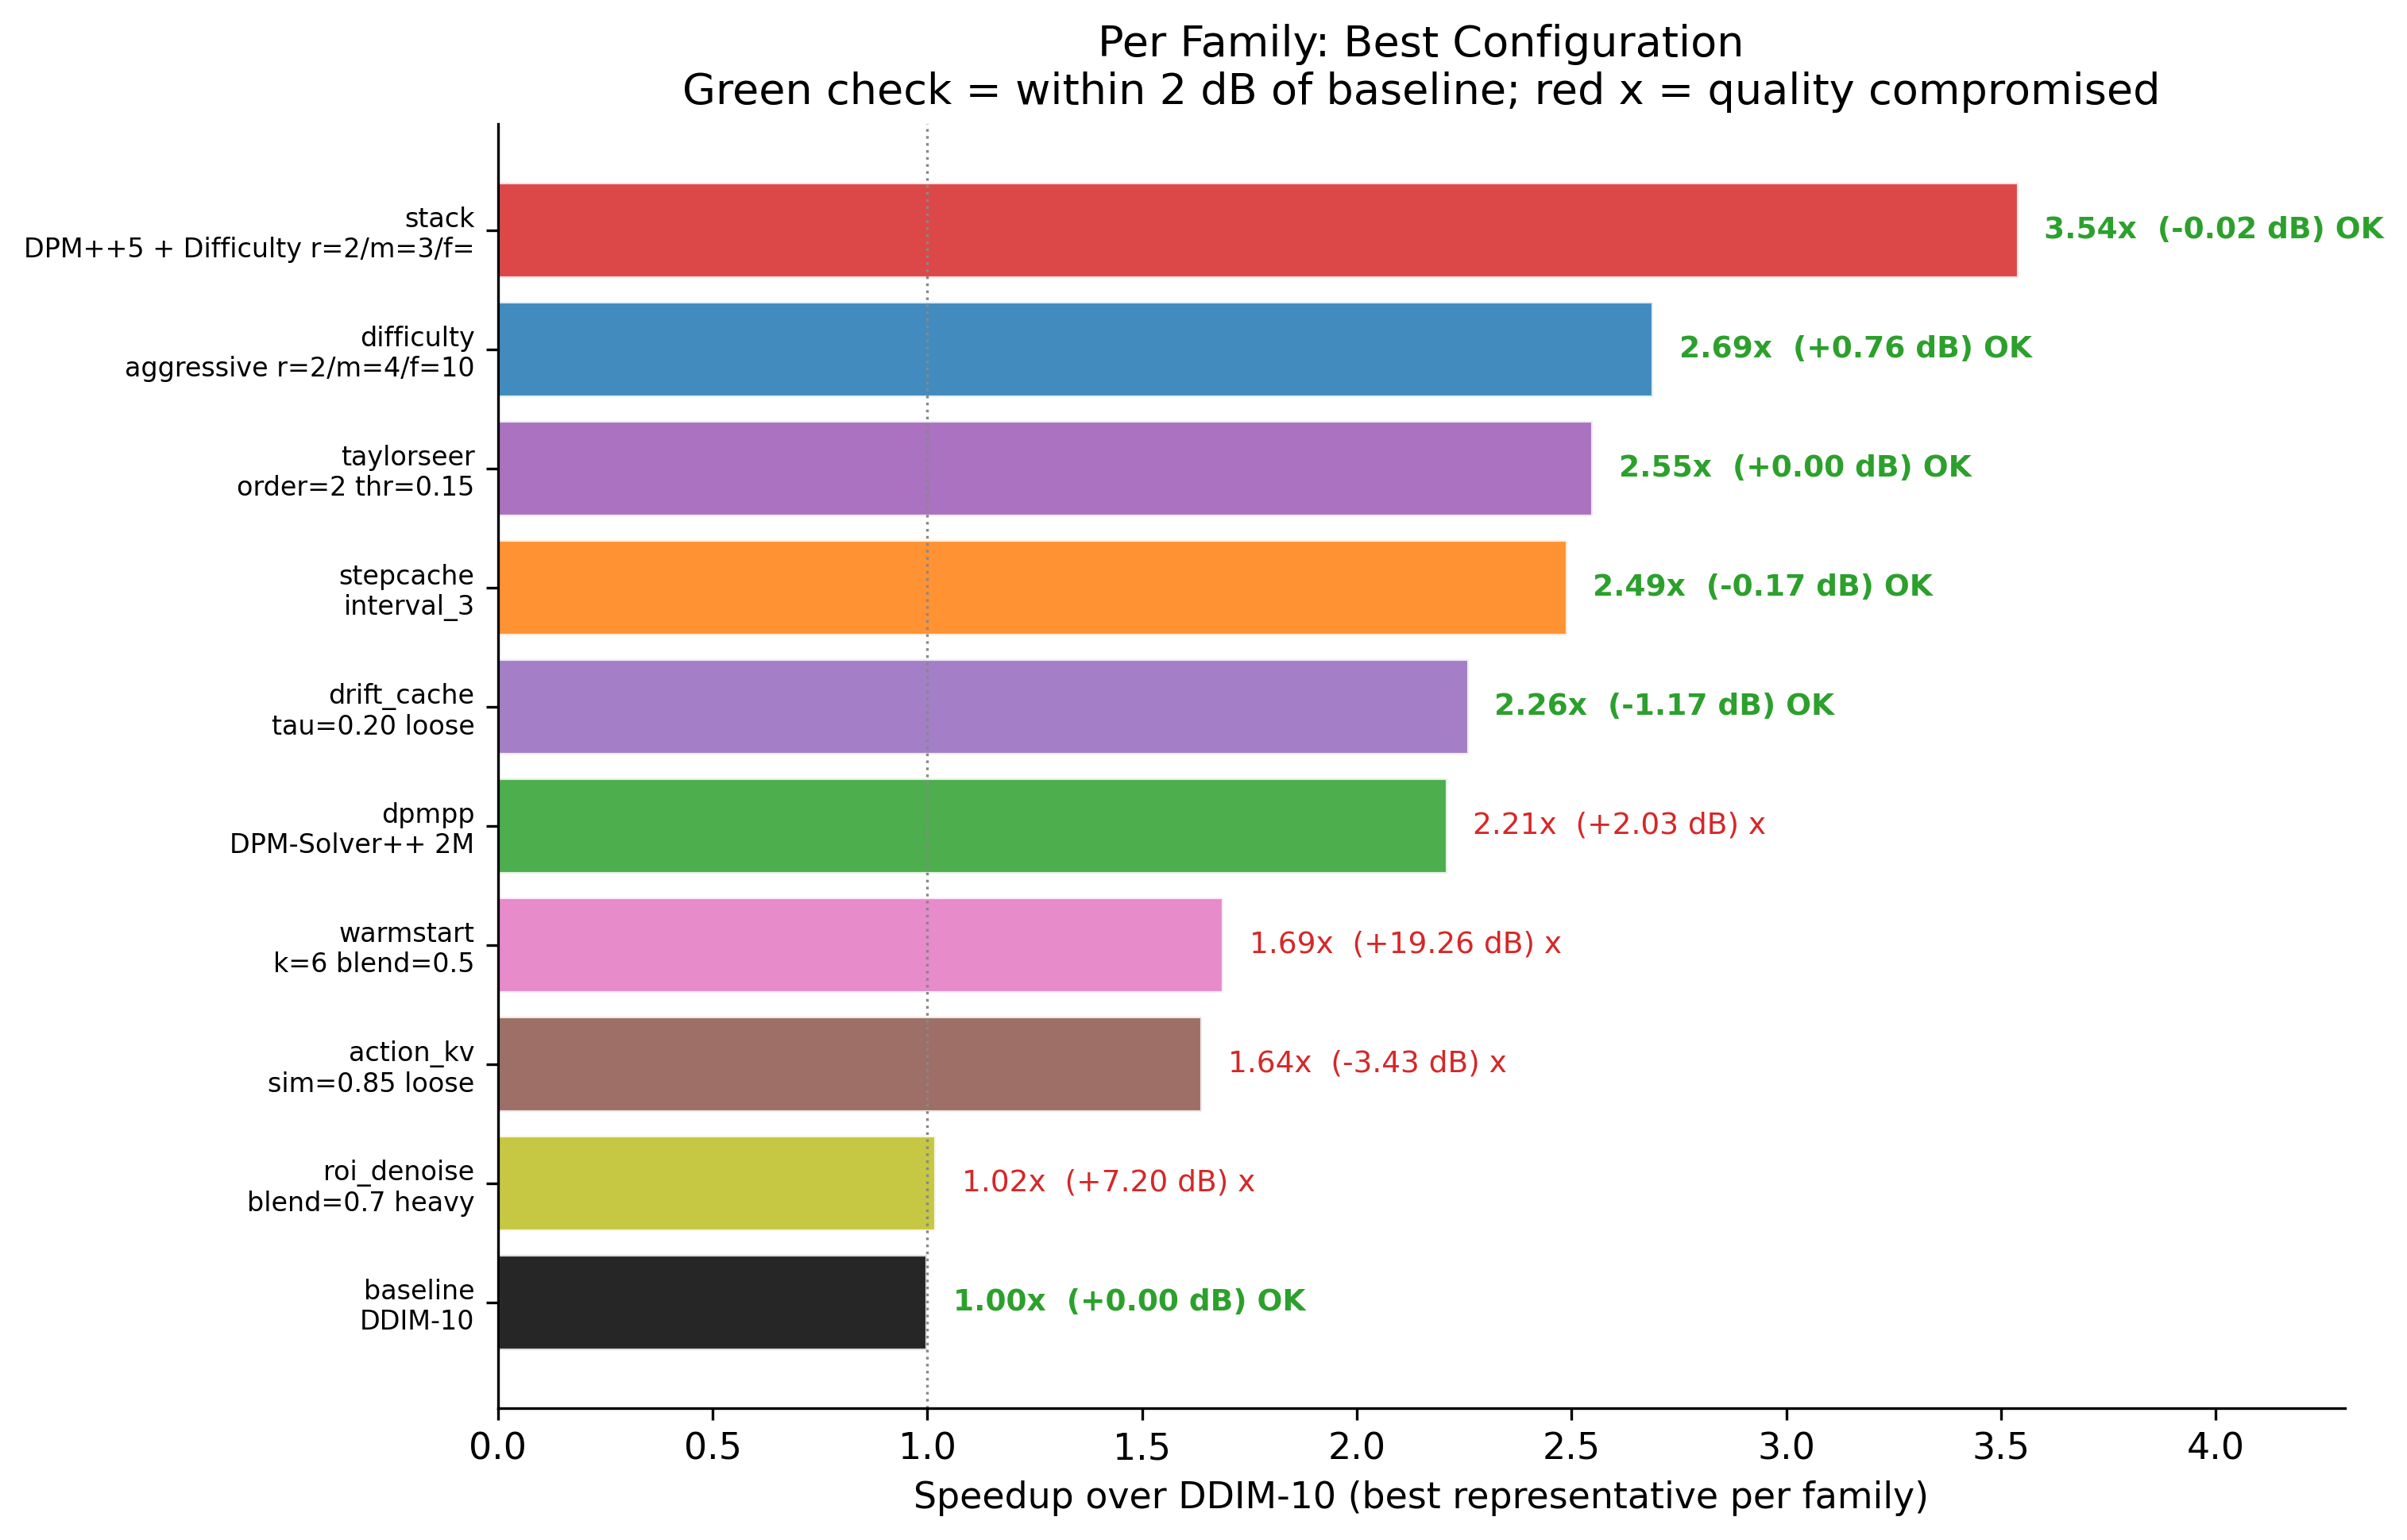
\includegraphics[width=\linewidth]{figures/per_family_pareto.png}
\caption{Best representative configuration per optimization family, sorted by speedup. Green checkmarks denote variants within $\pm 2$ dB of baseline self-coherence; red crosses denote quality-compromised variants.}
\label{fig:pareto}
\end{figure}

Figure~\ref{fig:pareto} compares the best representative per family. Five families clear the $|\Delta| < 2$ dB bar: our headline stack at 3.54$\times$, Difficulty aggressive at 2.69$\times$, TaylorSeer at 2.52$\times$, stepcache interval-3 at 2.49$\times$, and drift-cache at 2.26$\times$. Four families fail the quality bar: warm-start ($+19$ dB freeze), action-KV ($-21$ dB length collapse), ROI denoising ($+7$ dB without compute saving), and DPM-Solver++ alone ($+4.5$ dB at 950f, just outside the band, though visually sharp).

\subsection{Distribution Dominates Skip Count}
\label{sec:skip}

\begin{figure}[t]
\centering
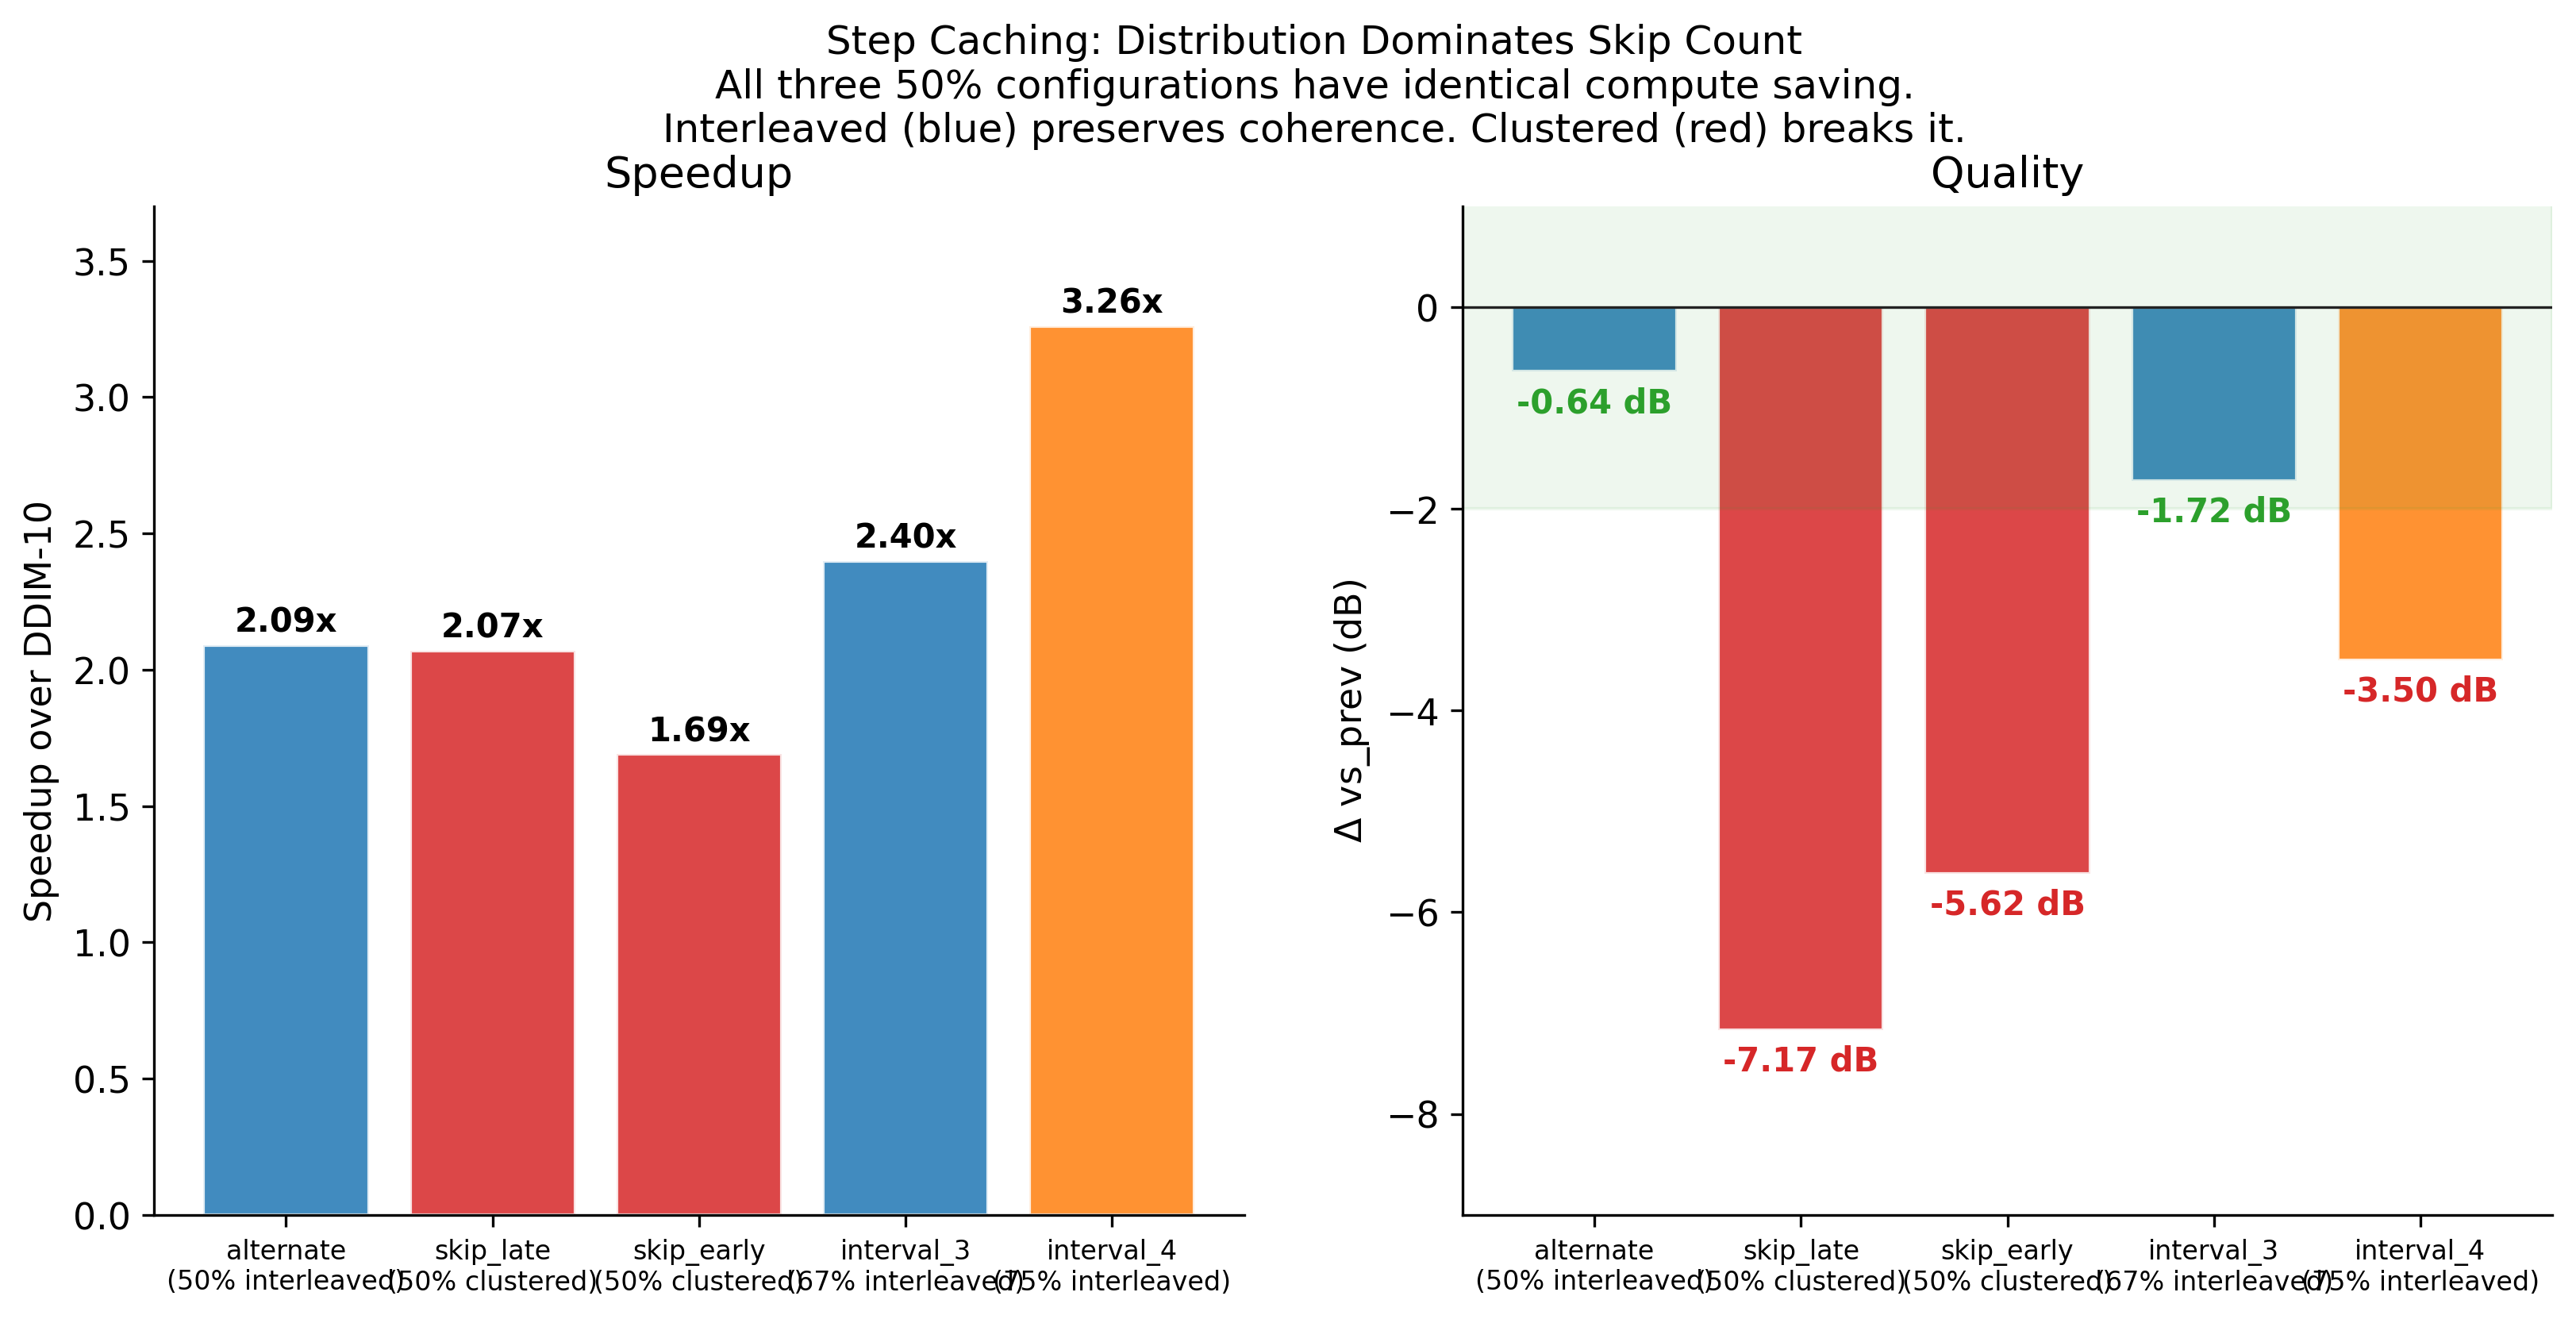
\includegraphics[width=\linewidth]{figures/skip_pattern_distribution.png}
\caption{Step caching skip pattern ablation at 32 frames. All three 50\% skip configurations save identical compute. Interleaved (\texttt{alternate}, blue) preserves coherence within $\pm 1$ dB. Clustered (\texttt{skip\_late}, \texttt{skip\_early}, red) collapses 5 to 7 dB.}
\label{fig:skip}
\end{figure}

A surprising finding from the step-caching ablation (Figure~\ref{fig:skip}) is that the \emph{distribution} of skipped steps matters more than the count. At identical 50\% skip rate, the \texttt{alternate} pattern (compute on noise idx 10, 8, 6, 4, 2; reuse on the rest) preserves coherence at $-0.64$ dB, while \texttt{skip\_late} (compute on the high-noise steps only) collapses to $-7.17$ dB and \texttt{skip\_early} (compute on low-noise only) to $-5.62$ dB. Interleaved skipping bounds the substitution noise per step; clustered skipping concentrates it on one end of the noise schedule and breaks trajectory formation.

This finding generalizes: in the megastack, TaylorSeer's prediction-eligible steps land on the late-noise end of the f=5 bucket, mirroring the \texttt{skip\_late} catastrophic pattern.

\subsection{All Configurations}

\begin{figure}[t]
\centering
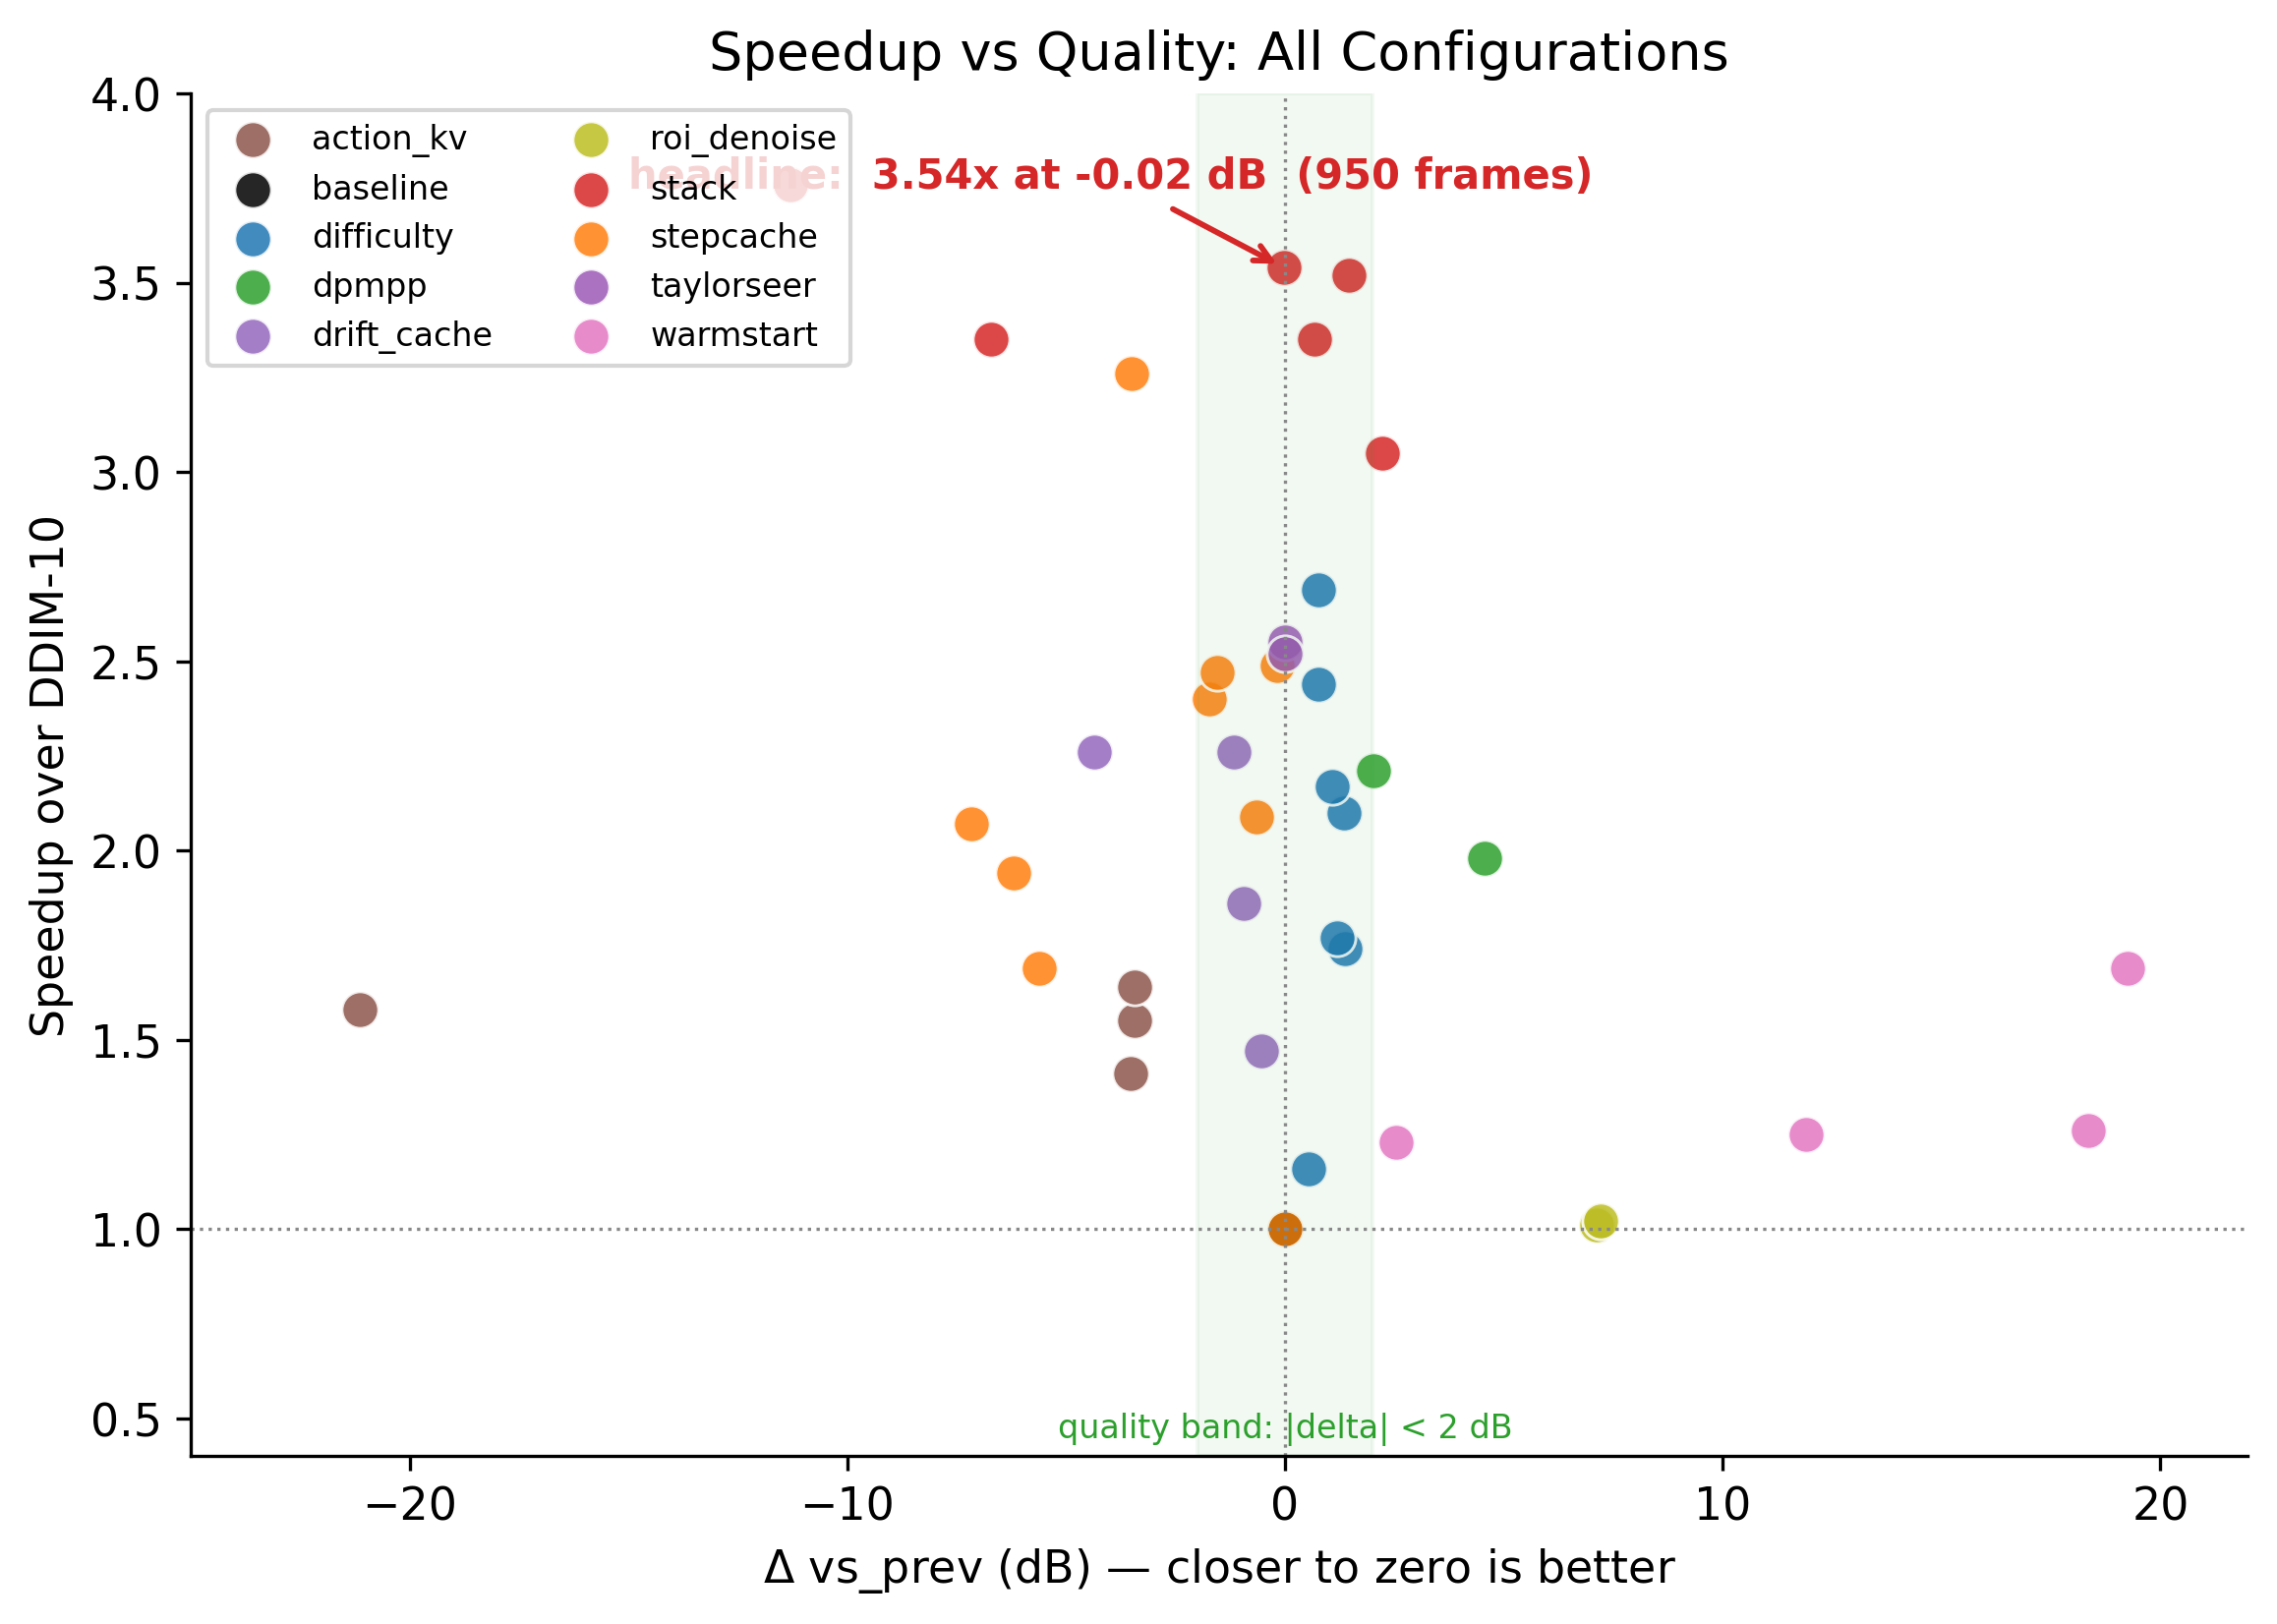
\includegraphics[width=\linewidth]{figures/speedup_vs_quality.png}
\caption{Every measured configuration plotted as a dot. X-axis: $\Delta$ vs\_prev (dB) versus DDIM-10 baseline. Y-axis: speedup. The pale green band marks the quality-preservation zone ($|\Delta| < 2$ dB). The headline stack sits at the top of the green band at 3.54$\times$ (annotated). Per-step substitution failures (action-KV at $-21$ dB, warm-start at $+19$ dB) define the catastrophic boundaries.}
\label{fig:scatter}
\end{figure}

Figure~\ref{fig:scatter} plots all 72 measured configurations. The headline annotation marks DPM++ $\times$ Difficulty at 3.54$\times$ inside the quality preservation band. The tail at $-21$ dB on the left is the action-KV catastrophe at 950 frames; the tail at $+19$ dB on the right is warm-start freezing.

\subsection{Failed Directions and Their Lessons}

We measured but rejected six families: KV-cache compression (FP8/INT4 substitution slower than baseline at batch=1, plus length collapse), action-conditional v reuse (constant $-3.4$ dB substitution cost at any threshold, $-21$ dB at length), warm-start latent anchoring (any blend $>0$ freezes), region-of-interest denoising (no compute saved without an attention-mask rewrite), torch.compile reduce-overhead mode (rotary library incompatibility), and INT4 weight quantization (dequantize overhead exceeds bandwidth saving at batch=1, $0.74\times$ slowdown). Each failure validates the broader claim: per-step substitution methods compound at length on autoregressive video.

%==================================================================
\section{Conclusion}
%==================================================================

We presented a 3.54$\times$ training-free speedup recipe for Open-Oasis 500M autoregressive Minecraft world model inference, validated across 950 real frames at $-0.02$ dB self-coherence. The recipe combines DPM-Solver++ 2M (a higher-order ODE solver halving the per-frame ceiling from 10 to 5 DDIM steps) with an action-magnitude bucket schedule that picks 2, 3, or 5 steps within the ceiling per frame from the free 25-dim Minecraft action signal. Our central empirical finding from 72 measured runs across 16 optimization families is that step-count reduction is autoregressive-safe while per-step substitution methods compound their error across length and crash 5 to 22 dB below baseline coherence. We further port TaylorSeer to autoregressive video with per-frame state reset, achieving 2.52$\times$ at 950 frames with zero validation failures, the first per-step skip method we measured to survive 950 frames at preserved quality. The action signal in the world model's input pipe is, to our knowledge, the first free per-frame difficulty signal exploited for adaptive diffusion compute. Future work will extend the recipe to other action-conditioned world models (Cosmos, MAGI, Matrix-Game 2.0) and integrate confidence-gated block prediction (CG-Taylor) to make per-step skipping safely stackable with the headline.

\bibliography{refs}

\end{document}
